\begin{frame}
	\frametitle{History}
	\begin{itemize}
		\item Founded in 2009
		\item Continuous growth in preferences 
		\item 3 seats won local elections (2010)
		\item 2.66 \% in parliament elections (2013)
		\item 4.78\% in European Parliament elections (2014)
		\item 21 seats gained in local elections (2014)
		\item Supported independent senators together with greens
	\end{itemize}
	
	% Lasst mir, bitte, erste mal ganz kurz Historie unserer Partei errinern. Die Partei wurde in 2009 gefunden. Seit der Zeit hatten wir ein Ständiges Wachsen von Preferenzen in Umfragen. Eine kleine Politische Abitur für uns ware die Wahl zum Arbegeordnetenhaus. Unserer Erfolg war leider nicht genugend um Abgeordente zu haben, aber wir sind jetzt offiziel von Staat finanziert. Das erlaubt uns mehr professionälle und merkbare Kampagne organisieren. Wir waren fast erfolgreich in der Europawahl, nur wegen dem Sperrklausel haben wir leider keienen Europaabgeordenten. Und wir zusammenarbeiten mit der Grünen in Senatwahlen, weil die Senatoren sind mit Mehreitswahl gewählt. Durch diese Kooperation konnten wir nach der letzten Wahl ein Klub im Senat zussamen mit Grünen und Unabhängigen gründen.
\end{frame}
\begin{frame}
	\frametitle{Organization}
	\begin{itemize}
		\item ca. 400 members
		\item Separate legislative, executive and judicuary branches
		\item Spokespeople for individual policy sections
		\item General forum comprised of all members
		\item Organisation units on geographical basis
		\item Transparent online forum
		\item Transparent accounting
	\end{itemize}
	
	
% Die Organisation der Partei ist bischen komplizierter. Wir haben unabhängige Organe, die arbeiten als Legislative, Exekutive und Judikative. Theoretisch begründet, wir wollen auf der Partei unsere Idee testen, die wir gern später auf dem Staat benutzen. Das System funktioniert vielleicht bischen byrokratisch, aber es hat ein Vorteil - die Partei war bis jetzt immer wirklich sparsam in vergleich zu anderen Tschechischen Parteien. Es nicht so einfach Geld zu verschwenden. Anderseits, wir haben kontinuelle Klagen gegen Byrokratie.
% Nächste sache - wir haben Themenbauftragte für jedes Thema die unseres Program behandelt. Die Person ist beantwortlich für Ausserungen zu aktuelle Ereignisen in dem Fach. Das System funktioniert vielleicht bischen wie in PP-Deutschland. Leider haben wir Probleme - die Partei ist relativ klein in Vergleich zur Deutschen PP, so manche Funktionen sind nicht besetzt.
% Wir selbstverständlich unterstutzen Basisdemokratie, so die höhste Entscheidungsrecht hat die Republikforum, als eine Versamlung von aller Mitglieder.
% Die Partei ist regionalbasiert. Aber ehrlich sagen, sie ist doch relativ zentalisiert. Die Regionen z.b. benutzen gemeinsames Bankkonto, Forum und haben gemeinsame Lobbyvorschriften. Eine Federalisierung ist kein Program sowohl für die Partei auch für den Staat.
% Die Hauptkommunikationsplatform ist leider immer ein Altes phpBB Forum. Was vielleicht überraschend ist, das Forum ist freizugänglich - so jeder, auch nicht Mitglieder, darf kommen. Wir haben Probleme mit Trolls, aber wir wollen zeigen, wie unsere Politik fuktioniert.
% Und wir haben transparente Finanzieurung.

\end{frame}
\begin{frame}
	\frametitle{Transparent accounting}
	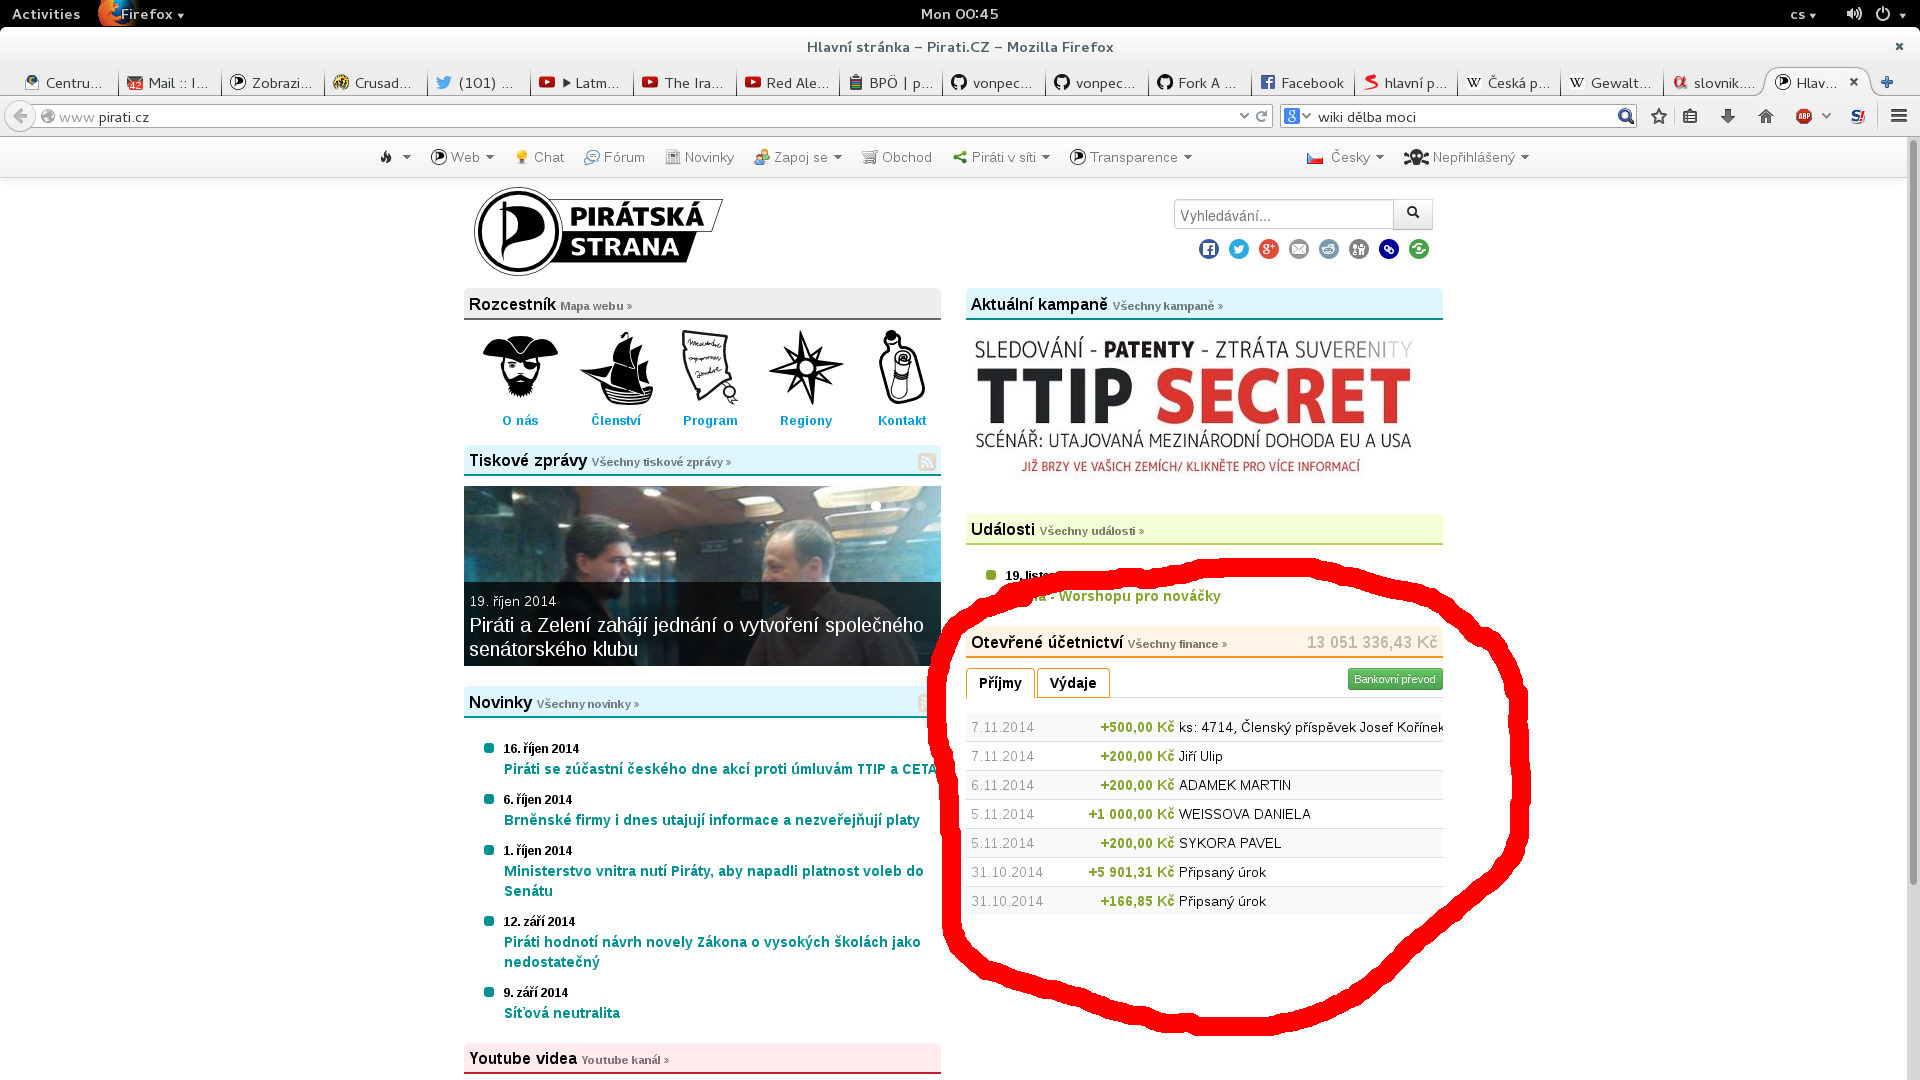
\includegraphics[scale=0.16]{piraticz.png}
% Das heist - wenn man klickt auf unseren webseite, sieht es so aus. Da kann man entscheiden, ob er Einkommen oder Ausgaben sehen will. Und es ist gleich klar, wer finanziert uns, und was wir mit dem Geld machen. 
\end{frame}
\begin{frame}
	\frametitle{Transparent accounting}
	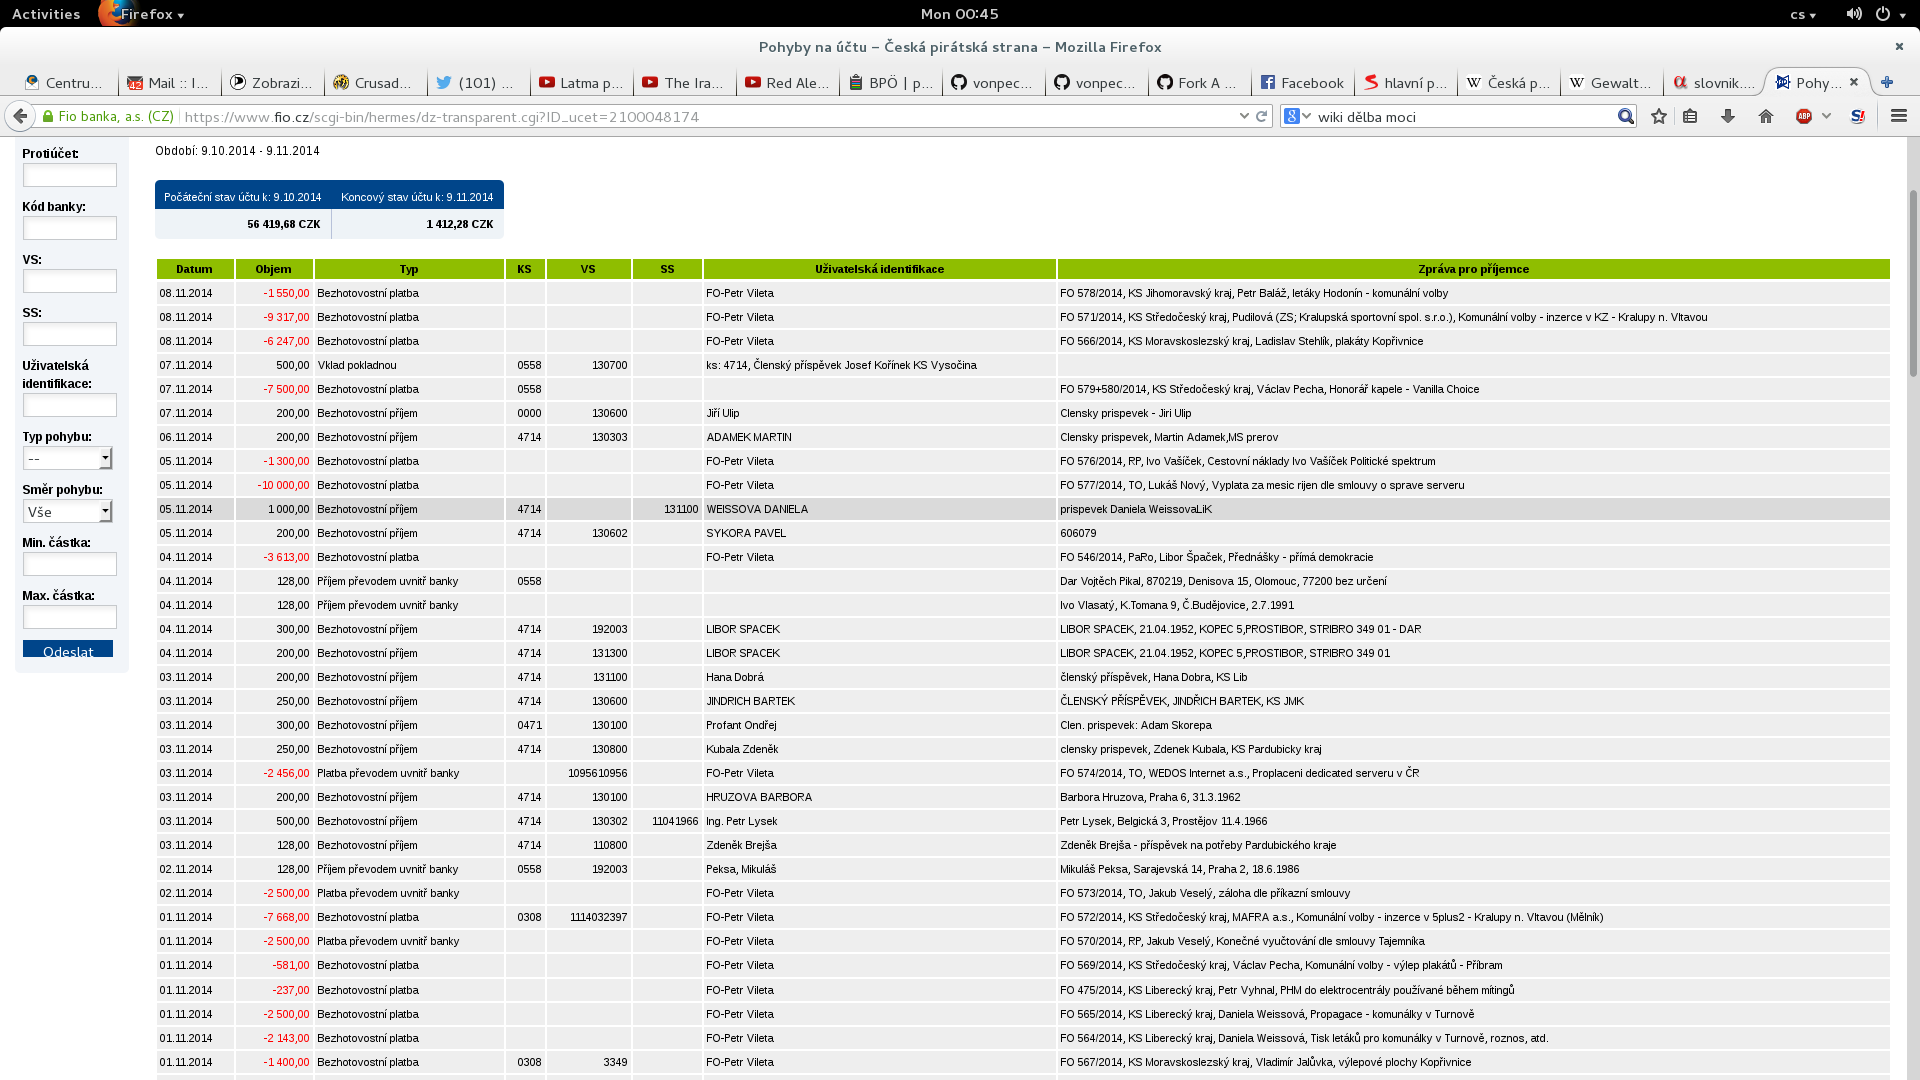
\includegraphics[scale=0.16]{fiocz.png}
% Man kann es auch losklicken, weil es ein Link direkt an der Webseite von der Bank führt. Sodass es kein Cheating ist. Alles ist selbstverständlich auch in den Akten von unseren Schatzmeister beschrieben. Und die Akten sind auch freizugänglich am Internet. Wir finden es als eiene tolle Massnahme gegen Korruption. In Zukunft möchten wir dieses System bei alle Parteien und auch Nichtregierungsorganisationen durchsetzen.
\end{frame}
\begin{frame}
	\frametitle{Policy}
	\begin{itemize}
		\item \textbf{Direct democracy}
		\item \textbf{Europe without borders and byrocracy}
		\item Freedom of speech
		\item Open access and open data
		\item Privacy
		\item Drug legalization
		\item Equality
		\item Transparency
		\item E-government
		\item Creative commons
		\item Internet freedom
		\item ...
	\end{itemize}
% Ihr seit Piraten und deswegen muss ich euch nicht Program von Piraten erklären. Die Piraten sind grenzlos und wir verstehen einander gut in der ganzen Welt. Also an der Stelle möchte ich mich nur auf die Unterschiede zwischen Tschechische und Österreichichsche Piratenpartei konzentrieren. Das, was uns leider trennt. Zum Glück, gibt es nur ein Paar beispiele. So - wenn wir über Basisdemokratie sprechen, meinen wir Direktdemokratie. Meinung der Mehrheit in Partei ist gegen Delegation von Stimmrecht, wie es z.b. in LiquidFeedback funktioniert. Wir möchten die Demokratie wirklich auf der Basis von Referenda wie in Schweiz gründen.
% Ich sage es hauptsächlich deswegen, weil ich möchte gern eine Basisdemokratie auf Europäische ebene sehen. Ich bin persönlich ein überzeugender Europäer. Ich kann persönlich gleich das alles, was ihr zu Europa in eurem Program habt, unterschreiben.  Aber Tschechien ist algemein mehr euroskeptisch in Vergleich zu Österreich. Es kann passieren, dass wir verschidene meinungen zu Europapolitik haben. Die Leute sind noch nicht auf Gründung eines Europäisches Staat vorbereitet. Und wir sind Demokraten, wir können nicht gegen Will von der Leute gehen. 
% Die Tschechische PP positioniert sich jetzt wie PPn von Grossbritanien und Schweden als mehr eurokritische. Ich möchte es ändern - aber dazu braucht man viele beispiele von guter zusammenarbeit zwischen Tschechien und nachbarländer - wie z.b. Österreich.
	
\end{frame}
\begin{frame}
	\frametitle{Activities}
	\begin{itemize}
		\item PirateLeaks, leak of copyright reform drafts, leak of internet censorship bill draft
		\item ACTA protests in 2012
		\item TTIP and CETA protests in 2014
		\item VyOseni music festival since 2011
		\item Free movie festival, 2013
		\item "Link is not a crime" long-term campaign
		\item "We play free music" long-term campaign
		\item Participative budgeting
		\item Presence at various venues related to our policies, press releases related to current issues

		%%http://www.pirati.cz/mo/verejnost/chronicles/start
		%%stanoviska
	\end{itemize}
\end{frame}

\begin{frame}
	\frametitle{International cooperation}
	\begin{itemize}
		\item Founding member of PPI, international conference with Amelia Andresdotter in 2010, PPI GA in 2012, PP-EU member
		\item Helped Berlin Pirates with campaign in 2011
		\item Mutual support with Saxon Pirates in 2013 (Bundestag in D, Abgeordnetenhaus in CZ)
		\item Helped Croatian pirates with campaign in 2013
		\item PP3 meeting in Saxony 2013 and Czechia 2014
	\end{itemize}
\end{frame}
%%stavime na neustale aktivite -> ukazat, co vse delame/delali jsme
% zduvodnit volebni vysledek historii + nezaspinenosti & touhou po zmene
